%% bare_conf.tex
%% V1.4b
%% 2015/08/26
%% by Michael Shell
%% See:
%% http://www.michaelshell.org/
%% for current contact information.
%%
%% This is a skeleton file demonstrating the use of IEEEtran.cls
%% (requires IEEEtran.cls version 1.8b or later) with an IEEE
%% conference paper.
%%
%% Support sites:
%% http://www.michaelshell.org/tex/ieeetran/
%% http://www.ctan.org/pkg/ieeetran
%% and
%% http://www.ieee.org/

%%*************************************************************************
%% Legal Notice:
%% This code is offered as-is without any warranty either expressed or
%% implied; without even the implied warranty of MERCHANTABILITY or
%% FITNESS FOR A PARTICULAR PURPOSE! 
%% User assumes all risk.
%% In no event shall the IEEE or any contributor to this code be liable for
%% any damages or losses, including, but not limited to, incidental,
%% consequential, or any other damages, resulting from the use or misuse
%% of any information contained here.
%%
%% All comments are the opinions of their respective authors and are not
%% necessarily endorsed by the IEEE.
%%
%% This work is distributed under the LaTeX Project Public License (LPPL)
%% ( http://www.latex-project.org/ ) version 1.3, and may be freely used,
%% distributed and modified. A copy of the LPPL, version 1.3, is included
%% in the base LaTeX documentation of all distributions of LaTeX released
%% 2003/12/01 or later.
%% Retain all contribution notices and credits.
%% ** Modified files should be clearly indicated as such, including  **
%% ** renaming them and changing author support contact information. **
%%*************************************************************************


% *** Authors should verify (and, if needed, correct) their LaTeX system  ***
% *** with the testflow diagnostic prior to trusting their LaTeX platform ***
% *** with production work. The IEEE's font choices and paper sizes can   ***
% *** trigger bugs that do not appear when using other class files.       ***                          ***
% The testflow support page is at:
% http://www.michaelshell.org/tex/testflow/



\documentclass[conference]{IEEEtran}
% Some Computer Society conferences also require the compsoc mode option,
% but others use the standard conference format.
%
% If IEEEtran.cls has not been installed into the LaTeX system files,
% manually specify the path to it like:
% \documentclass[conference]{../sty/IEEEtran}





% Some very useful LaTeX packages include:
% (uncomment the ones you want to load)


% *** MISC UTILITY PACKAGES ***
%
%\usepackage{ifpdf}
% Heiko Oberdiek's ifpdf.sty is very useful if you need conditional
% compilation based on whether the output is pdf or dvi.
% usage:
% \ifpdf
%   % pdf code
% \else
%   % dvi code
% \fi
% The latest version of ifpdf.sty can be obtained from:
% http://www.ctan.org/pkg/ifpdf
% Also, note that IEEEtran.cls V1.7 and later provides a builtin
% \ifCLASSINFOpdf conditional that works the same way.
% When switching from latex to pdflatex and vice-versa, the compiler may
% have to be run twice to clear warning/error messages.






% *** CITATION PACKAGES ***
%
%\usepackage{cite}
% cite.sty was written by Donald Arseneau
% V1.6 and later of IEEEtran pre-defines the format of the cite.sty package
% \cite{} output to follow that of the IEEE. Loading the cite package will
% result in citation numbers being automatically sorted and properly
% "compressed/ranged". e.g., [1], [9], [2], [7], [5], [6] without using
% cite.sty will become [1], [2], [5]--[7], [9] using cite.sty. cite.sty's
% \cite will automatically add leading space, if needed. Use cite.sty's
% noadjust option (cite.sty V3.8 and later) if you want to turn this off
% such as if a citation ever needs to be enclosed in parenthesis.
% cite.sty is already installed on most LaTeX systems. Be sure and use
% version 5.0 (2009-03-20) and later if using hyperref.sty.
% The latest version can be obtained at:
% http://www.ctan.org/pkg/cite
% The documentation is contained in the cite.sty file itself.






% *** GRAPHICS RELATED PACKAGES ***
%
\ifCLASSINFOpdf
\usepackage[pdftex]{graphicx}
  % declare the path(s) where your graphic files are
  % \graphicspath{{../pdf/}{../jpeg/}}
  % and their extensions so you won't have to specify these with
  % every instance of \includegraphics
  % \DeclareGraphicsExtensions{.pdf,.jpeg,.png}
\else
  % or other class option (dvipsone, dvipdf, if not using dvips). graphicx
  % will default to the driver specified in the system graphics.cfg if no
  % driver is specified.
  % \usepackage[dvips]{graphicx}
  % declare the path(s) where your graphic files are
  % \graphicspath{{../eps/}}
  % and their extensions so you won't have to specify these with
  % every instance of \includegraphics
  % \DeclareGraphicsExtensions{.eps}
\fi
% graphicx was written by David Carlisle and Sebastian Rahtz. It is
% required if you want graphics, photos, etc. graphicx.sty is already
% installed on most LaTeX systems. The latest version and documentation
% can be obtained at: 
% http://www.ctan.org/pkg/graphicx
% Another good source of documentation is "Using Imported Graphics in
% LaTeX2e" by Keith Reckdahl which can be found at:
% http://www.ctan.org/pkg/epslatex
%
% latex, and pdflatex in dvi mode, support graphics in encapsulated
% postscript (.eps) format. pdflatex in pdf mode supports graphics
% in .pdf, .jpeg, .png and .mps (metapost) formats. Users should ensure
% that all non-photo figures use a vector format (.eps, .pdf, .mps) and
% not a bitmapped formats (.jpeg, .png). The IEEE frowns on bitmapped formats
% which can result in "jaggedy"/blurry rendering of lines and letters as
% well as large increases in file sizes.
%
% You can find documentation about the pdfTeX application at:
% http://www.tug.org/applications/pdftex





% *** MATH PACKAGES ***
%
\usepackage{amsmath}
% A popular package from the American Mathematical Society that provides
% many useful and powerful commands for dealing with mathematics.
%
% Note that the amsmath package sets \interdisplaylinepenalty to 10000
% thus preventing page breaks from occurring within multiline equations. Use:
%\interdisplaylinepenalty=2500
% after loading amsmath to restore such page breaks as IEEEtran.cls normally
% does. amsmath.sty is already installed on most LaTeX systems. The latest
% version and documentation can be obtained at:
% http://www.ctan.org/pkg/amsmath





% *** SPECIALIZED LIST PACKAGES ***
%
%\usepackage{algorithmic}
% algorithmic.sty was written by Peter Williams and Rogerio Brito.
% This package provides an algorithmic environment fo describing algorithms.
% You can use the algorithmic environment in-text or within a figure
% environment to provide for a floating algorithm. Do NOT use the algorithm
% floating environment provided by algorithm.sty (by the same authors) or
% algorithm2e.sty (by Christophe Fiorio) as the IEEE does not use dedicated
% algorithm float types and packages that provide these will not provide
% correct IEEE style captions. The latest version and documentation of
% algorithmic.sty can be obtained at:
% http://www.ctan.org/pkg/algorithms
% Also of interest may be the (relatively newer and more customizable)
% algorithmicx.sty package by Szasz Janos:
% http://www.ctan.org/pkg/algorithmicx




% *** ALIGNMENT PACKAGES ***
%
%\usepackage{array}
% Frank Mittelbach's and David Carlisle's array.sty patches and improves
% the standard LaTeX2e array and tabular environments to provide better
% appearance and additional user controls. As the default LaTeX2e table
% generation code is lacking to the point of almost being broken with
% respect to the quality of the end results, all users are strongly
% advised to use an enhanced (at the very least that provided by array.sty)
% set of table tools. array.sty is already installed on most systems. The
% latest version and documentation can be obtained at:
% http://www.ctan.org/pkg/array


% IEEEtran contains the IEEEeqnarray family of commands that can be used to
% generate multiline equations as well as matrices, tables, etc., of high
% quality.


% *** SUBFIGURE PACKAGES ***
%\ifCLASSOPTIONcompsoc
%  \usepackage[caption=false,font=normalsize,labelfont=sf,textfont=sf]{subfig}
%\else
%  \usepackage[caption=false,font=footnotesize]{subfig}
%\fi
% subfig.sty, written by Steven Douglas Cochran, is the modern replacement
% for subfigure.sty, the latter of which is no longer maintained and is
% incompatible with some LaTeX packages including fixltx2e. However,
% subfig.sty requires and automatically loads Axel Sommerfeldt's caption.sty
% which will override IEEEtran.cls' handling of captions and this will result
% in non-IEEE style figure/table captions. To prevent this problem, be sure
% and invoke subfig.sty's "caption=false" package option (available since
% subfig.sty version 1.3, 2005/06/28) as this is will preserve IEEEtran.cls
% handling of captions.
% Note that the Computer Society format requires a larger sans serif font
% than the serif footnote size font used in traditional IEEE formatting
% and thus the need to invoke different subfig.sty package options depending
% on whether compsoc mode has been enabled.
%
% The latest version and documentation of subfig.sty can be obtained at:
% http://www.ctan.org/pkg/subfig




% *** FLOAT PACKAGES ***
%
%\usepackage{fixltx2e}
% fixltx2e, the successor to the earlier fix2col.sty, was written by
% Frank Mittelbach and David Carlisle. This package corrects a few problems
% in the LaTeX2e kernel, the most notable of which is that in current
% LaTeX2e releases, the ordering of single and double column floats is not
% guaranteed to be preserved. Thus, an unpatched LaTeX2e can allow a
% single column figure to be placed prior to an earlier double column
% figure.
% Be aware that LaTeX2e kernels dated 2015 and later have fixltx2e.sty's
% corrections already built into the system in which case a warning will
% be issued if an attempt is made to load fixltx2e.sty as it is no longer
% needed.
% The latest version and documentation can be found at:
% http://www.ctan.org/pkg/fixltx2e


%\usepackage{stfloats}
% stfloats.sty was written by Sigitas Tolusis. This package gives LaTeX2e
% the ability to do double column floats at the bottom of the page as well
% as the top. (e.g., "\begin{figure*}[!b]" is not normally possible in
% LaTeX2e). It also provides a command:
%\fnbelowfloat
% to enable the placement of footnotes below bottom floats (the standard
% LaTeX2e kernel puts them above bottom floats). This is an invasive package
% which rewrites many portions of the LaTeX2e float routines. It may not work
% with other packages that modify the LaTeX2e float routines. The latest
% version and documentation can be obtained at:
% http://www.ctan.org/pkg/stfloats
% Do not use the stfloats baselinefloat ability as the IEEE does not allow
% \baselineskip to stretch. Authors submitting work to the IEEE should note
% that the IEEE rarely uses double column equations and that authors should try
% to avoid such use. Do not be tempted to use the cuted.sty or midfloat.sty
% packages (also by Sigitas Tolusis) as the IEEE does not format its papers in
% such ways.
% Do not attempt to use stfloats with fixltx2e as they are incompatible.
% Instead, use Morten Hogholm'a dblfloatfix which combines the features
% of both fixltx2e and stfloats:
%
% \usepackage{dblfloatfix}
% The latest version can be found at:
% http://www.ctan.org/pkg/dblfloatfix




% *** PDF, URL AND HYPERLINK PACKAGES ***
%
\usepackage{url}
% url.sty was written by Donald Arseneau. It provides better support for
% handling and breaking URLs. url.sty is already installed on most LaTeX
% systems. The latest version and documentation can be obtained at:
% http://www.ctan.org/pkg/url
% Basically, \url{my_url_here}.




% *** Do not adjust lengths that control margins, column widths, etc. ***
% *** Do not use packages that alter fonts (such as pslatex).         ***
% There should be no need to do such things with IEEEtran.cls V1.6 and later.
% (Unless specifically asked to do so by the journal or conference you plan
% to submit to, of course. )


% correct bad hyphenation here
\hyphenation{op-tical net-works semi-conduc-tor}


\begin{document}
%
% paper title
% Titles are generally capitalized except for words such as a, an, and, as,
% at, but, by, for, in, nor, of, on, or, the, to and up, which are usually
% not capitalized unless they are the first or last word of the title.
% Linebreaks \\ can be used within to get better formatting as desired.
% Do not put math or special symbols in the title.
\title{Towards a Benchmark for the Maintainability Evolution of Industrial
  Software Systems}

% author names and affiliations
% use a multiple column layout for up to three different
% affiliations
\author{\IEEEauthorblockN{Till D{\"o}hmen}
\IEEEauthorblockA{VU University Amsterdam\\
Amsterdam, Netherlands\\
Email: t.r.doehmen@vu.nl}
\and
\IEEEauthorblockN{Davide Ceolin}
\IEEEauthorblockA{VU University Amsterdam\\
Amsterdam, Netherlands\\
Email: d.ceolin@vu.nl}
\and
\IEEEauthorblockN{Joost Visser}
\IEEEauthorblockA{Software Improvement Group\\
Amsterdam, Netherlands\\
Email: j.visser@sig.eu}
\and
\IEEEauthorblockN{Magiel Bruntink}
\IEEEauthorblockA{Software Improvement Group\\
Amsterdam, Netherlands\\
Email: m.bruntink@sig.eu}}

% conference papers do not typically use \thanks and this command
% is locked out in conference mode. If really needed, such as for
% the acknowledgment of grants, issue a \IEEEoverridecommandlockouts
% after \documentclass

% for over three affiliations, or if they all won't fit within the width
% of the page, use this alternative format:
% 
%\author{\IEEEauthorblockN{Michael Shell\IEEEauthorrefmark{1},
%Homer Simpson\IEEEauthorrefmark{2},
%James Kirk\IEEEauthorrefmark{3}, 
%Montgomery Scott\IEEEauthorrefmark{3} and
%Eldon Tyrell\IEEEauthorrefmark{4}}
%\IEEEauthorblockA{\IEEEauthorrefmark{1}School of Electrical and Computer Engineering\\
%Georgia Institute of Technology,
%Atlanta, Georgia 30332--0250\\ Email: see http://www.michaelshell.org/contact.html}
%\IEEEauthorblockA{\IEEEauthorrefmark{2}Twentieth Century Fox, Springfield, USA\\
%Email: homer@thesimpsons.com}
%\IEEEauthorblockA{\IEEEauthorrefmark{3}Starfleet Academy, San Francisco, California 96678-2391\\
%Telephone: (800) 555--1212, Fax: (888) 555--1212}
%\IEEEauthorblockA{\IEEEauthorrefmark{4}Tyrell Inc., 123 Replicant Street, Los Angeles, California 90210--4321}}

% use for special paper notices
%\IEEEspecialpapernotice{(Invited Paper)}

% make the title area
\maketitle

% As a general rule, do not put math, special symbols or citations
% in the abstract
\begin{abstract}
Software maintainability is influential to future costs of feature extensions, bug fixes and refactoring measures throughout the whole lifecycle of a system.
Therefore, software engineers are aiming at creating well maintainable systems and also at improving the maintainability of existing systems to counteract technical debt.
The Software Improvement Group (SIG) established an ISO/IEC 25010-based model to assess software maintainability using static code analysis, based on which systems from different industries and government organizations were evaluated and monitored over time.
Focus of this research is to use the metrics history from more than 1500 different systems, to investigate how software maintainability of different systems changes over time.
We found that current maintainability and volume are determinant for the average evolution speed of maintainability over time.
The findings can serve as benchmark to assess the maintainability improvement performance of a systems, as a indication of potential future improvements and risks and could serve as starting point for a maintainability prediction model.

{\em TODO: rewrite given current focus.}
\end{abstract}

% no keywords

% For peer review papers, you can put extra information on the cover
% page as needed:
% \ifCLASSOPTIONpeerreview
% \begin{center} \bfseries EDICS Category: 3-BBND \end{center}
% \fi
%
% For peerreview papers, this IEEEtran command inserts a page break and
% creates the second title. It will be ignored for other modes.
\IEEEpeerreviewmaketitle

\section{Introduction}
The maintainance of software is an important cost factor for organizations across all industries, making up approximately 40\% to 70\% of the total development costs of a software system~\cite{grubb2003software}.
Furthermore, research on the evolution of software has shown that recurring effort is needed to keep operational software functionally relevant and technically up-to-date~\cite{lehman1980programs}.  
Hence maintainability, the ``the degree of effectiveness and efficiency with which a product or system can be modified to improve it, correct it or adapt it to changes in environment, and in requirements''~\cite{iso25010}, is considered a key characteristic of software.

The {ISO 25010} definition of software quality characteristics, in particular maintainability, has given rise to measurement models that use properties of the source code comprising software systems.
One such measurement model, the SIG Maintainability Model~\cite{sig-maintainability-model}, which was first described by Heitlager et. al in 2007~\cite{heitlager2007practical}, is currently in operational use by the Software Improvement Group (SIG)\footnote{\url{http://www.sig.eu}}, a software consultancy based in Amsterdam, the Netherlands.
This model is capable of automatically determining a maintainability rating given a software system's source code and a (proprietary) benchmark database of previous measurements~\cite{alves2010deriving}.
The resulting maintainability ratings are expressed on a scale of 1 to 5 `stars', where a 3-star rating is calibrated to reflect a market-average maintainability.
The operational application of this model for a period of approximately 10 years has produced a significant set of data describing the evolution of maintainability of many industrial software systems.

This data set allows for the exploration of some questions regarding maintainability evolution, which we approach from the perspective of building a benchmark against which software systems can be compared.
In particular it is important to determine the base (change) rates of maintainability, i.e., the rates of change observed in the (benchmark) population prior to taking into account distinctive features, such as system size or age.

Knowing the base rates of maintainability evolution is necessary for the accurate interpretation of software measurement results~\cite{bruntink2015towards}.
Furthermore, rates of maintainability evolution are useful tools for estimation and planning of renovation and maintenance projects.
Most software systems will benefit from remaining at an already-high maintainability level, but what about systems that are currently poorly maintainable?
The question is when it would be feasible and beneficial to try and renovate such systems, and when it would be better to leave them as-is.

Concretely, in this paper we will discuss the following research questions:
\begin{enumerate}
\item \textit{What is the base rate of maintainability change?}
\item \textit{What properties of software correlate with the rates of maintainability change?}
\item \textit{How could a benchmark of maintainability evolution be constructed?}
\end{enumerate}

First, we provide some background information on the software metrics that were used in the research in Section~\ref{sec:background}. Then we describe the process of data collection in Section~\ref{sec:DataCollection}, followed by an exploratory data analysis in Section~\ref{sec:analysis}. Section~\ref{sec:Discussion} discusses the data analysis results from the perspective of the questions listed above. Related work is reflected in Section~\ref{sec:related}. Finally, Section~\ref{sec:conclusion} concludes and discussed opportunities for future work.

%%% Local Variables:
%%% mode: latex
%%% TeX-master: "IWSM-Mensura-2016"
%%% End:

\section{Data Collection}
\label{sec:DataCollection}

\subsection{Context}

The basis for our benchmark is maintainability data collected for a large sample of projects by the SIG as part of their Software Monitoring \cite{kuipers2004portfoliomonitoring}.
This service consists of two parts: standardized analyses of the maintainability of the source code, and customized advice to reduce project risks.

For the first part of the service the source code of a software project is analyzed by the tooling of SIG on a regular (usually weekly) basis.
The input of this tooling is a snapshot of the source code of the software project on a certain time; the output is a database containing facts about the system in the form of software metrics.
This data is made available to both the consultancy team inside SIG as well as the development team of the project in a two-stage process.
After an initial analysis the data is stored in an acceptance environment in which sanity checks are performed before the data is put into a production environment.
One of the sanity checks is related to changes in the volume of the system, making sure that large changes in volume are always inspected manually. 

In the second part of the service this software metric data extracted from the source code is augmented by other data-resources and analyzed by the consultancy team to determine the current risks of the software project and formulate possible mitigation actions.
The results of the analyses are first validated with key-personnel of the client, after which the results of this process are presented to the client in reporting sessions, which normally take place on a monthly or quarterly basis. 

The important thing to note here is that the results of the analyses, as well as the data collection process, are validated on a regular basis with the persons developing and managing the software project.
Because of this, anomalies in the source code or the configuration of the tooling are detected and handled in a timely manner.
In addition, note that all of these projects are monitored because there is an interest in the quality of the software.

\subsection{Process}

As explained above, the analyses of source code follows a standardized process.
The first step in this process is the creation of the initial configuration for the analyses tooling.
This configuration specifies core aspects of the software project such as the technologies used and the main components. 

In addition, for each technology the configuration specifies which parts of the source code are dedicated to testing, which parts of the source code are generated, and which parts of the source code consist of external libraries not maintained by the development team.
Stripping out these categories of code leaves only the code that is maintained by the development team and is part of the running system, i.e., the \emph{production code} \cite{alves2011categories}. 

To identify these different categories the consultant creating the configuration uses the guidelines outlined in the SIG/T\"UViT Evaluation Criteria Trusted Product Maintainability~\cite{sig-maintainability-model} as a basis.
These guidelines allow the inclusion of, amongst others, source code files, generated code undergoing manual modifications, and data schemas, while explicitly excluding artifacts such as data files, binary
files, and documentation from the measurement scope. 

After creating the initial configuration the monitoring of the source code is a largely automated, two-phased process.
In the first phase the analyses is run and the results are stored in an acceptance environment.
Automated sanity checks are run in this environment to check for unusual changes in the received source code, amongst others based on large differences in the volume of the code for a specific technology or the addition of new technologies. 

If all sanity checks pass, the data is moved from the acceptance environment to the production environment.
When one of the sanity checks fails, the Monitor Control Center (MCC) is alerted.
This control center is staffed with (at least) one consultant which investigates the causes of the failed sanity check, and contacts the development team at the client if needed.
Based on the cause of the failure, the delivered snapshot can, for example, be rejected or the configuration can be adapted before the values of the analyses are placed in the production environment. 

In addition, the results of the analyses are stored in a data-warehouse called the Software Analysis Warehouse (SAW).
The SAW contains the software metrics for each software project for each snapshot of the source code received from the client.
Note that the storage takes place after the automated sanity checks, which means that rudimentary validation has already taken place.
However, during the manual validation or analyses of the data small changes can be made to the scope, for example to include a library initially marked as ``not maintained by the team'' because changes have been made to this source code.
These changes in configuration are taken into account when analyzing the next snapshot of the system, but are typically not applied retrospectively.  

%%% Local Variables:
%%% mode: latex
%%% TeX-master: "IWSM-Mensura-2016"
%%% End:

\section{Analysis}
\label{sec:analysis}
This chapter will describe the analysis approach and subsequently present the results. From a business perspective the prediction interval of one quarter year is of special interest, that is why some parts of the analysis will be based on a time period of 13 weeks.

\subsection{Data Cleaning}
The data was cleaned from snapshots which showed more churn than 90\% of total lines of code, code churn which was not following the logarithmic law of size/relative churn ratio (using a gracious threshold removing only 2\% of the most deviating snapshots) and two systems were excluded based on manual inspection. Noise in churn data was most likely caused by re-scoping of the analyzed code base, file or folder renaming, initial data imports into the software analysis warehouse and code generators. Because churn data should, for this study, represent human effort, snapshots with unrealistic high churn values were excluded.

\subsection{Extraction of Transitions}

\begin{figure}[htbp!]
  \label{schema}
  \centering
  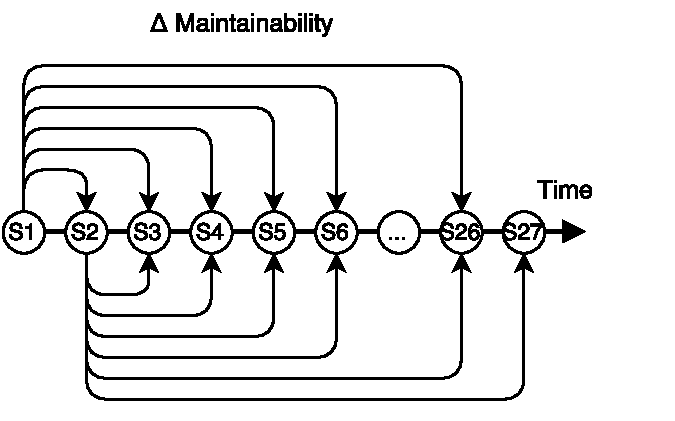
\includegraphics[width=0.50\textwidth]{figs/extraction.pdf}
  \caption{State transition extraction schema for first two snapshots. Circles denote snapshots. Every arrow connecting two snapshots denotes an extracted transition.}
\end{figure}

To investigate the change of maintainability, each snapshots was extracted together with maximum 25 proceeding snapshots belonging to the same system. With a given median snapshot distance of 7 days and an average of 13 snapshots per system we expect that this set of snapshots cover at least a time span of 13 weeks for most systems. Then, for each series, maintainability deltas and time deltas between first and n-th proceeding snapshot were determined. Every transition was saved together with information about it's start state and it's end state. Code change related metrics were commulated over all snapshots between start and end. Figure 1 visualizes this extraction process and Table \ref{data_points} shows the resulting extracted features.
\begin{table}[htbp!]
\caption{Attributes of Extracted Transition Data Points}
\begin{tabular}{l  p{5.2cm}}
  \hline			
  Property & Description \\ \hline
  Snapshot ID & ID of start snapshot \\
  Maintainability & Maintainability of start snapshot\\ 
  Volume & Volume of start snapshot\\ 
  Maintainability delta & \(\Delta\)(Maintainability start, Maintainability end)\\
  Time delta & \(\Delta\)(Date start, Date end)\\
  LOC start & Total lines of code of start snapshot\\ 
  LOC end & Total lines of code of end snapshot\\ 
  Changed lines & Commulative changed lines between start and end snapshot \\
  Code Churn & Commulative code churn between start and end snapshot \\ 
  Deleted lines & Commulative deleted lines between start and end snapshot \\ \hline
\end{tabular}
\label{data_points}
\end{table}

After excluding transitions which do not show any code changes $\sim$300000 data points were left for the following analysis.

\subsection{Maintainability Change Base Rate}

\subsection{System Grouping}
We preferred using cluster center as starting point for the grouping process instead of an equally spaced grid on the data. This gives us the advantage of groups which have small inner-group and large between-group variances.
The number of cluster was chosen to be 125, which is approximately the number of all combinations of maintainability and volume in 0.5 point steps and is as well in line with the Kanti's rule of thumb \cite{kanti1979multivariate} of \(k\approx\sqrt{50000/2}\approx158\). 

Clustering was performed with Weka~\cite{hall2009weka} using k-means clustering with Euclidean distances based on maintainability and volume.
Due to the correlation between maintainability and volume, not every combination of volume and maintainability is equally supported by data. This does though not lead to substantial problems for later analysis.

Subgroups of systems were built around the cluster center, by selecting the 5\% closest (Euclidean distance) data points to each cluster center. This leads to 125 subgroups of \textasciitilde15000 elements each. It is to note that same data points can be assigned to multiple subgroups if they are lying close to each other. The groups are not disjoint on purpose, in that way each subgroups can contain a larger amount of data points which will be essential for getting stable quantile estimation in the next step. The resulting group center are additionally not significantly different from the previously determined cluster center.

\subsection{Maintainability/Volume Aware Change Rate}
Maintainability change was analyzed for each of the previously determined groups separately, over time, leading to a plot as in Figure 2. The dark points mark the weekly 10th and 90th percentiles and the red lines are quantile regression lines on the same percentiles. The upper red line marks the maintainability improvement of the 'top-performers' and the lower line the deterioration of the 'worst-performer'. The plot shows data for the first 13 weeks only, while the quantile regression line was fitted on the full data set which contains support for up to 26 weeks to over-fitting on the 13 week interval. Two different quantile regression models were fitted to the data: \(percentile\sim sqrt(time)\) and \(percentile\sim sqrt(time)+time\). Both lead to comparable sum of squared error rates over all systems, but the latter model was chosen because of the additional linear term, which creates more realistic fits corner cases in which the change rate is very low or changes direction. 
The cone spanning between top-performer and worst-performer describes the 80\% confidence interval in which a system of that type will end up during the next 13 weeks, based on observations in the given dataset. This can already be considered as a useful approach to benchmark the quality improvement performance of a specific system.
\begin{figure}[htbp!]
  \label{cone}
  \centering
  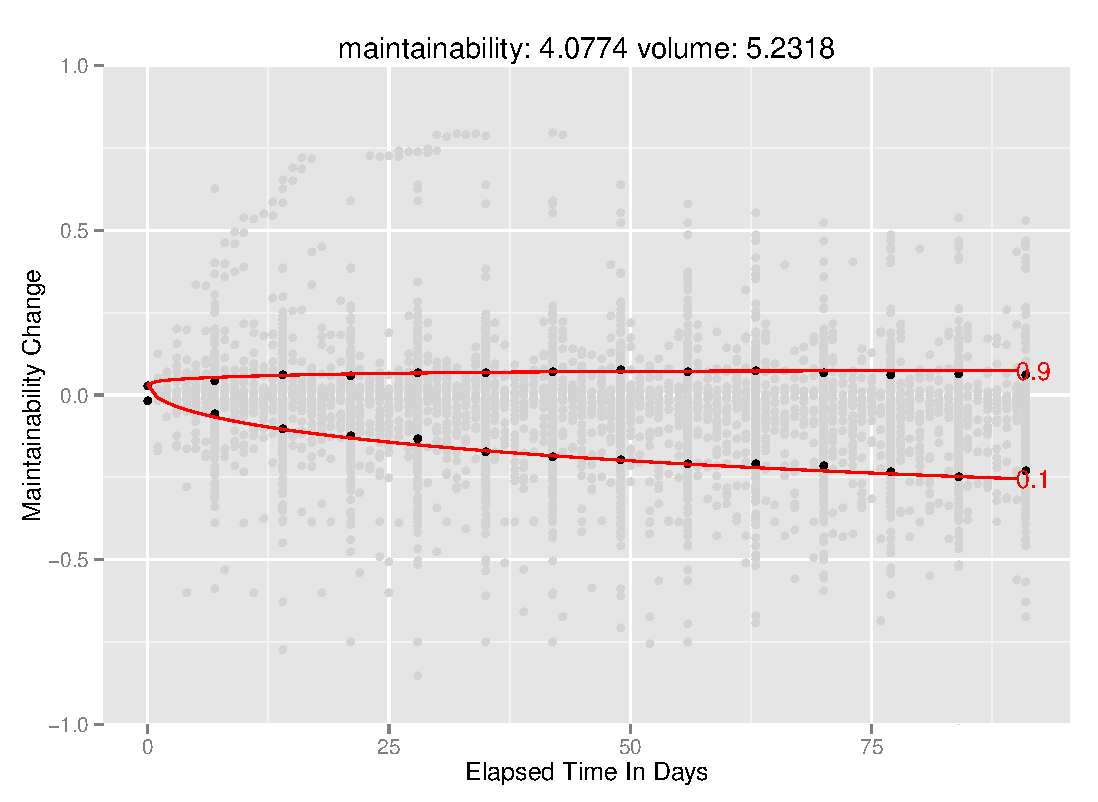
\includegraphics[width=0.5\textwidth]{figs/graph_m_4v_5.pdf}
  \caption{Maintainability change quantile regression (10th and 90th percentile, \(percentile\sim sqrt(time)+time\)) over 13 weeks, for a specific group of systems around cluster center m=4.0774, v=5.2318}
\end{figure}
However, first visual inspection of the resulting plots for each group showed significantly different cones, which leads to the conclusion that hypothesis H1 can be confirmed. Further objective was to explain the difference, by maintainability and volume of the respective groups. 
The ambitions to fit a linear regression model on the quantile regression parameter of the upper and lower line, did not lead to promising results. 
Subsequently, a model was fitted on the upper (90th) and lower (10th) maintainability change percentiles in the 13th week.  
Linear models for the lower quantile leads to high significance and a high R-square value. Thus, the lower boundary for maintainability change in 13 weeks can be expressed with a simple linear model. Same models on the upper quantile lead though to non-significant results. Further analysis explained the weakness of the first approach and revealed a change in trend at \(maintainability*volume>13.5\). 
Subsequently, both regions were analyzed separately, leading to significant models for both regions. We can thus confirm H2 as well. See Table \ref{correlations} for detailed outcomes of the analysis with and without the interaction term. 
\begin{table}[htbp!]
\caption{Correlation Analysis Results}
\begin{tabular}{l  l l p{0.7cm}}
  \hline			
  Percentile & Formula & R-sq. & sign.\\ \hline
  10th & \(perc\sim v+m\) & 0.78 & \textless 0.001\\
  10th & \(perc\sim v+m+v*m\) & 0.92 & \textless 0.001\\ 
  90th (MxV\textless13.5) & \(perc\sim v+m\) & 0.72 & \textless 0.001\\
  90th (MxV\textless13.5) & \(perc\sim v+m+v*m\) & 0.75 & \textless 0.01\\
  90th (MxV\textgreater=13.5) & \(perc\sim v+m\) & 0.77 & \textless 0.001\\
  90th (MxV\textgreater=13.5) & \(perc\sim v+m+v*m\) & 0.82 & \textgreater 0.05\\
\end{tabular}
\label{correlations}
\end{table}

Because of acceptable r-squared values and residual plot for model with and without interaction terms, we decided to present the more intuitive interpretable results for the linear models without interaction terms (see Table \ref{results}).
\begin{table}[htbp!]
\centering
\caption{Linear Regression Models on Upper and Lower Bound for Maintainability Change over 13 Weeks}
\begin{tabular}{l  l  l p{1.2cm}}
  \hline			
  Percentile & Intercept & M & V\\ \hline
  10th & 0.253116 & -0.020066 & -0.085102\\ 
  90th (left) & -0.115953 & 0.039481 & 0.024165\\
  90th (right) & 0.414851 & -0.147388 & 0.056140\\
\end{tabular}
\label{results}
\end{table}

\subsection{Benchmark}
objectivity, reliability, validity.
average quantile in their group
Because objective of this study is not to make a point prediction for one specific system, but to reveal an underlying trend regardless of how one individual projects behaves. One specific system might improve in one week and deteriorate or stay the same in the next week, which depends on various factors which are certainly not completely covered by the current data set. But we hypothesize that maintainability and volume are the two main driving factors for maintainability improvement potential. To measure the improvement potential we want to determine the upper 90\% quantile of maintainability improvement in a subgroup, which is based on maintainability and volume rankings. This would reflect the amount of improvement which the 'top-performer' of certain subgroup achieved and thus implicitly mark an upper bound for improvement of a specific system category. We want to point out that maintainability and volume are not the only possible factors influencing the improvement of maintainability, but the hypotheses give us a starting point to develop a set of methods, which can be used to investigate different factors in future work as well.

%%% Local Variables:
%%% mode: latex
%%% TeX-master: "IWSM-Mensura-2016"
%%% End:

\section{Discussion}
\label{sec:Discussion}


%%% Local Variables:
%%% mode: latex
%%% TeX-master: "IWSM-Mensura-2016"
%%% End:

\section{Related Work}
\label{sec:related}
Software metrics are quantitative descriptions of software systems and related processes and cover concepts like size, complexity, maintainability and code change. Mining in software metrics can be regarded as part of Mining Software Repositories (MSR) \cite{kagdi2007survey}, whereas MSR generally makes also use of meta data from CVS or bug-tracking systems and analyzes software on code level, which is not scope of our study. Studies dealing with metric data, showed that data pre-processing is an essential first step, because of several reasons. First, many metrics are log-normal distributed and require a transformation, second, they are often multi-collinear and, third, the data sets are often noisy and contain outlier. An often mentioned approach to solve the problem of multi-collinearity is Principal Component Analysis (PCA) as proposed by~\cite{dick2004data}, \cite{nagappan2006mining} and \cite{nikora2003understanding}. Noise in metrics datasets is a problem which is often seen as a thread to validity, but is not frequently addressed \cite{liebchen2010data}. Approaches to noise and outlier detection in software engineering datasets are existing~\cite{lep2013noise}, but to our knowledge there is not no general approach established. Mining in software metrics was applied to different problems in the past, e.g., failure prediction~\cite{nagappan2006mining} \cite{finlay2011mining} and complexity evolution~\cite{nikora2003understanding}.

Studies concerned with effort estimation are often working on open datasets like ISBSG which contain metrics, project meta data and the actual effort values for a large set of systems. Effort estimations on those datasets make use of machine learning techniques ranging from simple linear regression and decision trees to multilayer perceptron neural networks and support vector machines \cite{dejaeger2012data}. Additionally there are analogy-based estimation techniques, which show "a renewed presence since 2008" \cite{fernandez2014potential} and comparison-based techniques. Hill et al. \cite{hill2010practical} describes the comparison-based approach as a technique which uses the median effort for a comparable subset of other systems as estimator. The results of those methods are easy comprehensible and comprehensibility plays according to Dejaeger et al. an "important role in acceptance of the model in a business setting" \cite{dejaeger2012data}.

Effort estimation models focus either on total effort or on effort for specific phases or specific development types. In the ISBSG dataset, development types are discriminated into new development, enhancement and re-development and all have the underlying phases planning, specification, design, building, testing and deployment \cite{lenarduzzi2014estimating}. Other literature proposes a further discrimination of enhancement or maintenance effort into the subcategories corrective, adaptive, perfective and preventive maintenance, where the latter one is defined as preventative change to prevent malfunctions or to improve maintainability \cite{grubb2003software}.
Studies we could identify which were concerned with maintainability effort prediction did either not focus on preventative maintenance \cite{hayes2004metrics}, \cite{basgalupp2012predicting}, \cite{leung2002estimating} or did not use comparison-based approaches \cite{jorgensen1995experience}, whereas Niessink et al. mention the analogy-based analysis as promising \cite{niessink1997predicting}.

Based on the related literature we are of the opinion that a comparison-based approach for effort estimation of preventative maintenance on a non-ISBSG dataset can be a valuable contribution to the current state of research.

\section{Conclusions and Future Work}
\label{sec:conclusion}
We have explored various factors related to maintainability improvement effort, as preliminary work towards a more comprehensive prediction model for such effort. We have focused specifically on current values and change patterns of volume and maintainability. Starting from the hypotheses formulated in Section III, we have been able to establish that the possible amount of maintainability improvement can be predicted based on a linear model, depending on maintainability and volume of a system. Additionally we could establish a model quantifying the required effort for maintainability improvement in terms of daily code churn.

Apart from volume and maintainability, more factors need to be studied before an accurate prediction model for maintainability improvement effort can be obtained. These may include environmental factors (e.g. development method, developer skills, industry segment, etc) or additional technical factors (e.g. architectural styles, dependencies on third-party components, unit test quality). Also, we intend to make our analysis more detailed by distinguishing development phases (e.g. initial development versus maintenance), drilling down to the level of components or even files, and cross-linking with actual effort registrations.


% conference papers do not normally have an appendix


% use section* for acknowledgment
%\section*{Acknowledgment}

% An example of a floating figure using the graphicx package.
% Note that \label must occur AFTER (or within) \caption.
% For figures, \caption should occur after the \includegraphics.
% Note that IEEEtran v1.7 and later has special internal code that
% is designed to preserve the operation of \label within \caption
% even when the captionsoff option is in effect. However, because
% of issues like this, it may be the safest practice to put all your
% \label just after \caption rather than within \caption{}.
%
% Reminder: the "draftcls" or "draftclsnofoot", not "draft", class
% option should be used if it is desired that the figures are to be
% displayed while in draft mode.
%
%\begin{figure}[!t]
%\centering
%\includegraphics[width=2.5in]{myfigure}
% where an .eps filename suffix will be assumed under latex, 
% and a .pdf suffix will be assumed for pdflatex; or what has been declared
% via \DeclareGraphicsExtensions.
%\caption{Simulation results for the network.}
%\label{fig_sim}
%\end{figure}

% Note that the IEEE typically puts floats only at the top, even when this
% results in a large percentage of a column being occupied by floats.


% An example of a double column floating figure using two subfigures.
% (The subfig.sty package must be loaded for this to work.)
% The subfigure \label commands are set within each subfloat command,
% and the \label for the overall figure must come after \caption.
% \hfil is used as a separator to get equal spacing.
% Watch out that the combined width of all the subfigures on a 
% line do not exceed the text width or a line break will occur.
%
%\begin{figure*}[!t]
%\centering
%\subfloat[Case I]{\includegraphics[width=2.5in]{box}%
%\label{fig_first_case}}
%\hfil
%\subfloat[Case II]{\includegraphics[width=2.5in]{box}%
%\label{fig_second_case}}
%\caption{Simulation results for the network.}
%\label{fig_sim}
%\end{figure*}
%
% Note that often IEEE papers with subfigures do not employ subfigure
% captions (using the optional argument to \subfloat[]), but instead will
% reference/describe all of them (a), (b), etc., within the main caption.
% Be aware that for subfig.sty to generate the (a), (b), etc., subfigure
% labels, the optional argument to \subfloat must be present. If a
% subcaption is not desired, just leave its contents blank,
% e.g., \subfloat[].


% An example of a floating table. Note that, for IEEE style tables, the
% \caption command should come BEFORE the table and, given that table
% captions serve much like titles, are usually capitalized except for words
% such as a, an, and, as, at, but, by, for, in, nor, of, on, or, the, to
% and up, which are usually not capitalized unless they are the first or
% last word of the caption. Table text will default to \footnotesize as
% the IEEE normally uses this smaller font for tables.
% The \label must come after \caption as always.
%
%\begin{table}[!t]
%% increase table row spacing, adjust to taste
%\renewcommand{\arraystretch}{1.3}
% if using array.sty, it might be a good idea to tweak the value of
% \extrarowheight as needed to properly center the text within the cells
%\caption{An Example of a Table}
%\label{table_example}
%\centering
%% Some packages, such as MDW tools, offer better commands for making tables
%% than the plain LaTeX2e tabular which is used here.
%\begin{tabular}{|c||c|}
%\hline
%One & Two\\
%\hline
%Three & Four\\
%\hline
%\end{tabular}
%\end{table}


% Note that the IEEE does not put floats in the very first column
% - or typically anywhere on the first page for that matter. Also,
% in-text middle ("here") positioning is typically not used, but it
% is allowed and encouraged for Computer Society conferences (but
% not Computer Society journals). Most IEEE journals/conferences use
% top floats exclusively. 
% Note that, LaTeX2e, unlike IEEE journals/conferences, places
% footnotes above bottom floats. This can be corrected via the
% \fnbelowfloat command of the stfloats package.


% trigger a \newpage just before the given reference
% number - used to balance the columns on the last page
% adjust value as needed - may need to be readjusted if
% the document is modified later
%\IEEEtriggeratref{8}
% The "triggered" command can be changed if desired:
%\IEEEtriggercmd{\enlargethispage{-5in}}

% references section

% can use a bibliography generated by BibTeX as a .bbl file
% BibTeX documentation can be easily obtained at:
% http://mirror.ctan.org/biblio/bibtex/contrib/doc/
% The IEEEtran BibTeX style support page is at:
% http://www.michaelshell.org/tex/ieeetran/bibtex/
\bibliographystyle{IEEEtran}
% argument is your BibTeX string definitions and bibliography database(s)
\bibliography{IEEEabrv,IWSM-Mensura-2016}
%
% <OR> manually copy in the resultant .bbl file
% set second argument of \begin to the number of references
% (used to reserve space for the reference number labels box)
% that's all folks
\end{document}

%%% Local Variables:
%%% mode: latex
%%% TeX-master: t
%%% End:
